\documentclass[letterpaper]{book}
\usepackage[utf8]{inputenc}

\usepackage[left=1.5cm, right=1.5cm, top=2cm, bottom=2cm]{geometry}

% Math typesetting
\usepackage{amsfonts}
\usepackage{amssymb}
\usepackage{amsmath}

% General font and language packages
\usepackage[english]{babel}
\usepackage{helvet}
\usepackage{courier}

% Tables and typesetting
\usepackage{setspace}
\linespread{2}
\frenchspacing
\setlength{\pdfpagewidth}{8.5in}
\setlength{\pdfpageheight}{11in}

% Packages for handling code blocks
\usepackage{listings}
\lstset{
  backgroundcolor=\color{white},
  basicstyle=\linespread{1}\footnotesize\ttfamily
}

% Package for drawing Finite Automata
\usepackage{tikz}
\usetikzlibrary{arrows,automata,positioning}

\title{Applications of Automata and Formal Language Theory}
\author{Alexander L. Hayes}
\date{September 2018}


\begin{document}

\maketitle

\chapter{Crash Course in \LaTeX}

This \textit{will not} make you a pro at the art of typesetting.

This \textit{will provide} you with a brief overview of how to use the language for typesetting material often covered in ``Theory of Computation", like formal proofs and automata.

\section{Boilerplate}

Let's start simple and introduce ourselves with a ``hello-world"-like example where we create the basic structure of a \TeX file. Depending on your platform, create a new \texttt{main.tex} document and add the following to the file.

When you compile this document to create a \texttt{.pdf}, it should be fairly clear which parts translate into the outputs.

\begin{lstlisting}[language=TeX]
\documentclass{article}
\usepackage[utf8]{inputenc}

\title{Learning \LaTeX}
\author{Alexander L. Hayes}

\begin{document}
\maketitle

\section{Introduction}

Hello world.

\end{document}
\end{lstlisting}

We can practice with some of the examples from Michael Sipser, \textit{Introduction to the Theory of Computation, Third Edition}. This deterministic finite automata may be seen at Figure 1.4 on page 34, and is approximately reproduced below.

\setlength{\tabcolsep}{12pt}
\renewcommand{\arraystretch}{1.5}

\begin{center}
\begin{tabular*}{\textwidth}{ @{\extracolsep{\fill}} | c c |}
  \hline
  Image & \LaTeX \\
  \hline
  {\centering
  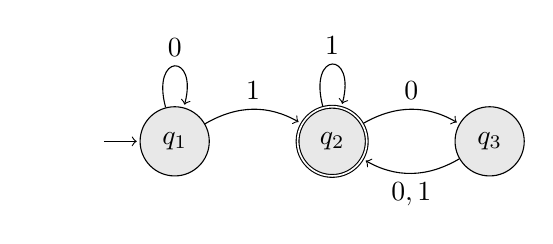
\begin{tikzpicture}[shorten >=1pt,node distance=2cm,auto]

    \tikzstyle{every initial by arrow}=[text=white,->]
    \tikzstyle{every state}=[fill={rgb:black,1;white,10}]

    \node[state,initial]    (q_1)                 {$q_1$};
    \node[state,accepting]  (q_2) [right of=q_1]  {$q_2$};
    \node[state]            (q_3) [right of=q_2]  {$q_3$};

    \path[->]
    (q_1) edge [loop above] node  {$0$}   (   )
          edge [bend left]  node  {$1$}   (q_2)
    (q_2) edge [loop above] node  {$1$}   (   )
          edge [bend left]  node  {$0$}   (q_3)
    (q_3) edge [bend left]  node  {$0,1$} (q_2);
  \end{tikzpicture}
  }
  &
  {\centering
  \begin{lstlisting}[language=TeX]

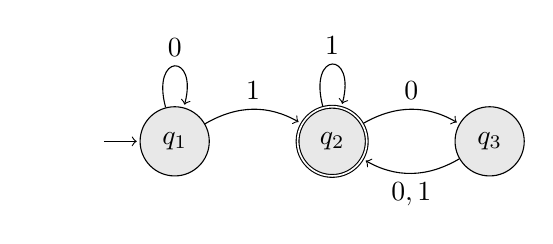
\begin{tikzpicture}[shorten >=1pt,node distance=2cm,auto]
  \tikzstyle{every initial by arrow}=[text=white,->]
  \tikzstyle{every state}=[fill={rgb:black,1;white,10}]

  \node[state,initial]    (q_1)                 {$q_1$};
  \node[state,accepting]  (q_2) [right of=q_1]  {$q_2$};
  \node[state]            (q_3) [right of=q_2]  {$q_3$};

  \path[->]
  (q_1) edge [loop above] node  {$0$}   (   )
        edge [bend left]  node  {$1$}   (q_2)
  (q_2) edge [loop above] node  {$1$}   (   )
        edge [bend left]  node  {$0$}   (q_3)
  (q_3) edge [bend left]  node  {$0,1$} (q_2);
\end{tikzpicture}
  \end{lstlisting}
  }
  \\
  \hline
\end{tabular*}
\end{center}

The next example comes from Figure 1.8 on page 37.

\begin{center}
\begin{tabular*}{\textwidth}{ @{\extracolsep{\fill}} | c c |}
  \hline
  Image & \LaTeX \\
  \hline
  {\centering
  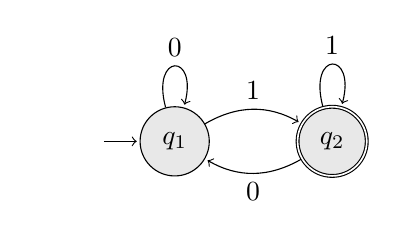
\begin{tikzpicture}[shorten >=1pt,node distance=2cm,auto]

    \tikzstyle{every initial by arrow}=[text=white,->]
    \tikzstyle{every state}=[fill={rgb:black,1;white,10}]

    \node[state,initial]    (q_1)                 {$q_1$};
    \node[state,accepting]  (q_2) [right of=q_1]  {$q_2$};

    \path[->]
    (q_1) edge [loop above] node  {$0$}   (   )
          edge [bend left]  node  {$1$}   (q_2)
    (q_2) edge [loop above] node  {$1$}   (   )
          edge [bend left]  node  {$0$}   (q_1);
  \end{tikzpicture}
  }
  &
  {\centering
  \begin{lstlisting}[language=TeX]

  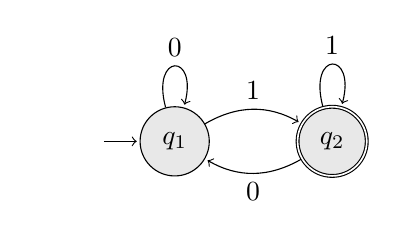
\begin{tikzpicture}[shorten >=1pt,node distance=2cm,auto]

    \tikzstyle{every initial by arrow}=[text=white,->]
    \tikzstyle{every state}=[fill={rgb:black,1;white,10}]

    \node[state,initial]    (q_1)                 {$q_1$};
    \node[state,accepting]  (q_2) [right of=q_1]  {$q_2$};

    \path[->]
    (q_1) edge [loop above] node  {$0$}   (   )
          edge [bend left]  node  {$1$}   (q_2)
    (q_2) edge [loop above] node  {$1$}   (   )
          edge [bend left]  node  {$0$}   (q_1);
  \end{tikzpicture}
  \end{lstlisting}
  }
  \\
  \hline
\end{tabular*}
\end{center}


\end{document}
